\documentclass[11pt,onecolumn]{IEEEtran}
\usepackage{diagbox}
\usepackage{graphicx}
\usepackage{amsmath}
\usepackage{amsfonts}
\usepackage{algpseudocode}
% \usepackage{algorithm}
\usepackage{subfigure}
\usepackage{tikz}
\usepackage{epsfig}
\usepackage{cite}
\usepackage[linesnumbered,ruled]{algorithm2e}

\newtheorem{theorem}{Theorem}
\newtheorem{proposition}{Proposition}
\newtheorem{definition}{Definition}
\newtheorem{lemma}{Lemma}
\newtheorem{corollary}{Corollary}
\newtheorem{example}{Example}


\renewcommand{\ae}[1]{{\color{red}{#1}}}
\newcommand{\my}[1]{{\color{blue}{#1}}}
\newcommand{\old}[1]{{\color{green}{#1}}}
\newcommand{\pur}[1]{{\color{purple}{#1}}}





\begin{document}     
\title{Prediction Uncertainty Based On Classification Agianst Unmodelled Input Space}
\author{Xiaozhe Gu\\Energy Research Institute (ERI@N), Singapore }

\maketitle

\section{Random Forest for Separating the space}
In this section, we propose a decision tree that can be used to separate regions that higher data density from other such regions by sparse regions in which most error could exist. One important reason we choose a decision tree classifier rather than other machine learning classifiers (e.g., neural networks) is that we do not need to sample data points for the empty space which can be very hard in high dimension space.
\subsection{Decision Tree Construction}

A commonly used criterion (or purity function) for choosing the best cut is the Gini impurity.  Gini impurity is a measure of how often a randomly chosen element from the set would be incorrectly labeled if it was randomly labeled according to the distribution of labels in the subset.  
\begin{align*}
I_G( p)=\sum_{k=1}^Kp_k(1-p_k)=1-\sum_{k=1}^K p_k^2\\
\end{align*}
, where $p_k$ denotes the fraction of items labeled $k$ in the set. In our case,  we are only interested in separating the training samples and the empty space, and the impurity of a subspace can be calculated as follows
\begin{align*}
& I_G(\mathcal R)=1-\left(\frac{\mathbb R}{\mathbb R+\mathbb E}\right)^2 -\left(\frac{\mathbb E}{\mathbb R+\mathbb E}\right)^2\\
\end{align*}
Here $\mathbb R$ and $\mathbb E$ denote the number of training samples and samples representing empty space  in region $\mathcal R$.   Suppose we cut $\mathcal R$ into two subspaces $\mathcal R_L(i,s)$ and $\mathcal R_R(i,s)$ by feature i and value s, then new Gini impurity  for the left child and right child can be calculated as follows


\begin{figure}[h]
    \centering
    \caption{Tree Representation}
    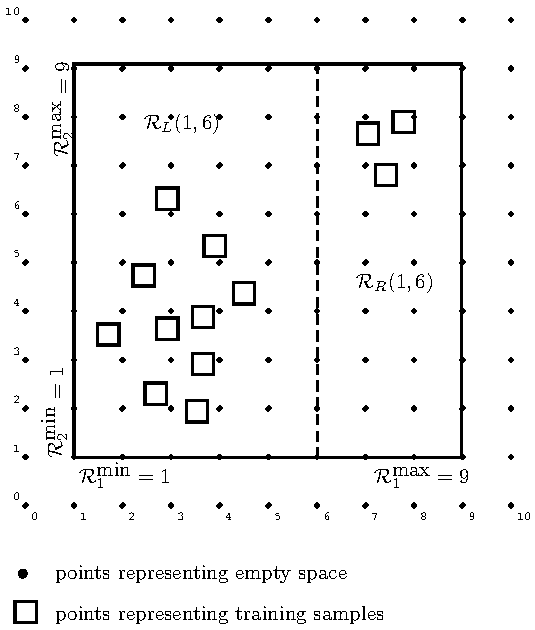
\includegraphics[scale=1]{image/split_example.pdf} 
    \end{figure}

\begin{align*}
IG_L(i,s)=1-\left(\frac{\mathbb R_L(i,s)}{\mathbb R_L(i,s)+\mathbb E_L}\right)^2-\left(\frac{\mathbb E_L}{\mathbb R_L(i,s)+ \mathbb E_L}\right)^2\\
\mathbb E_L=\mathbb E\times \left(\frac{s- \mathcal R^{\mbox{min}}_i}{\mathcal R^{\mbox{max}}_i-\mathcal R^{\mbox{min}}_i}\right)\\
IG_R(i,s)=1-\left(\frac{\mathbb  R_R(i,s)}{\mathbb  R_R(i,s)+\mathbb  E_R}\right)^2-\left(\frac{\mathbb  E_R}{\mathbb R_R(i,s)+\mathbb  E_R}\right)^2\\
\mathbb E_R=\mathbb E\times \left(\frac{\mathcal R_i^{\mbox{max}}-s}{\mathcal R_i^{\mbox{max}}-\mathcal R_i^{\mbox{min}}}\right)\\
\end{align*}
In the above equation,  $\mathbb R_L(i,s)$ and $\mathbb R_R(i,s)$  denote the number of training samples in the region $\mathbb R$ has  $X_i\leq s$ and $X_i\geq s$, respectively. $\mathcal R^{\mbox{min}}_i$ and  $\mathcal R^{\mbox{max}}_i$ denote the lower and upper bound of dimension i for region $\mathcal R$. Since the data points representing the empty space are assumed to be uniformed distributed among $\mathbb R$, then $\mathbb E_L$ and $\mathbb E_R$  are in  proportion to $s- \mathcal R^{\mbox{min}}_i$ and $\mathcal R_i^{\mbox{max}}-s$, respectively.
After the region $\mathbb R$ is divided into $\mathbb R_L(i,s)$ and $\mathbb R_R(i,s)$, the Gini impurity is updated as follows.

\begin{align*}
IG_{\mbox{split}}(i,s)=\frac{\mathbb R_L(i,s)+\mathbb E_L}{\mathbb R+ \mathbb E}IG_L(i,s)+\frac{\mathbb R_R+ \mathbb E_R}{\mathbb E+\mathbb R}IG_R(i,s)
\end{align*}
The decision tree will select to cut the space into subspaces  that minimizes the  Gini impurity.
\begin{align*}
i,s=\arg \min_{i,s} IG_{\mbox{split}}(i,s)
\end{align*}

  \begin{figure}[h]
    \centering
    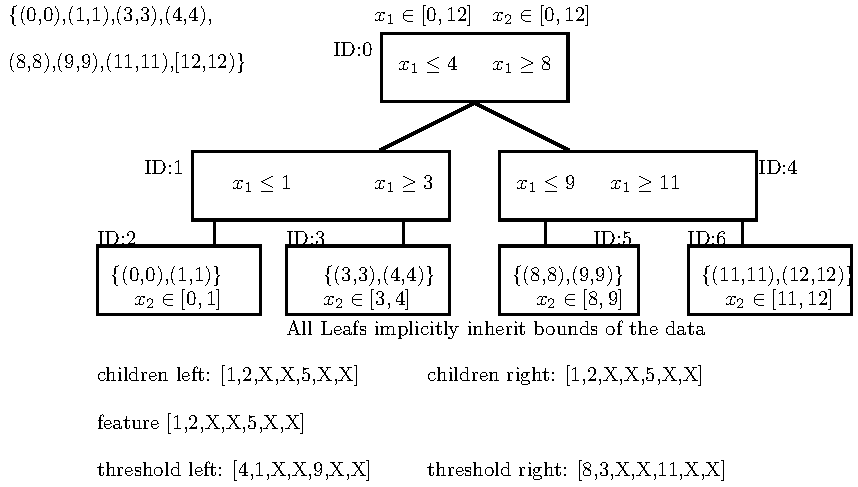
\includegraphics[scale=1]{image/tree.pdf} 
    \caption{Tree Representation}
    \label{fig:ExampleTree1}
    \end{figure}

  \begin{figure}[h!]
    \centering
    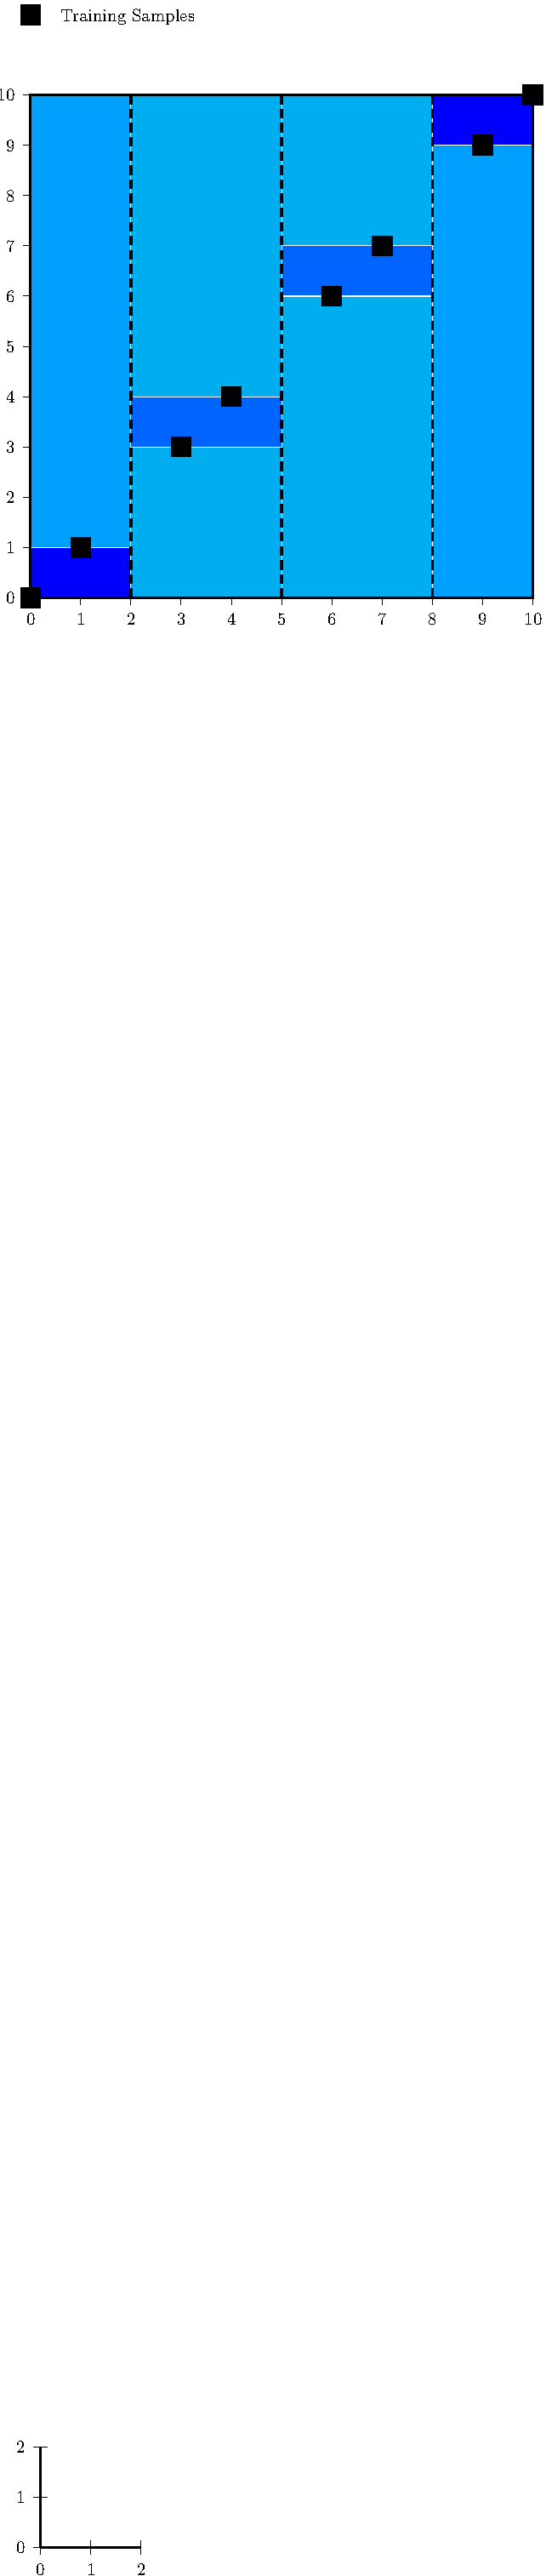
\includegraphics[scale=0.7]{image/rec.pdf} 
    \caption{Hyperrectangle}
    \label{fig:hyperrectangle}
    \end{figure}

\subsection{Inference}
After the tree is built, the initial region $\mathcal R$ will be divided into multiple hyperrectangle. In Figure~\ref{fig:ExampleTree1}, we show an example of a constructed tree for 2-d training samples  $X=\{(0,0),(1,1),(3,3),(4,4),(6,6),(7,7),(9,9),(10,10)\}$.  The initial region that covers training samples is $\mathcal R=[0,10]^2$ and its volume is $\mathcal R.vol=100$. We also assume  that infinite number of data points representing the empty space are uniformly distributed among $\mathcal R$ with weight $\frac{\mathbb R}{100}$. Thus, the total weighted number of empty points is equal to $\mathbb E=\mathbb R=10$.  


The tree divides $\mathcal R$ into four rectangles $\mathcal R_i,~i\in\{1,2,3,4\}$ by cut axis 1 at $\{2,5,8\}$.  Thus, the proportion of training samples in the four rectangles are $\frac{2}{2+2},\frac{2}{2+3},\frac{2}{2+3},\frac{2}{2+2}$, respectively.

Since axis 2 is not split, we can further divided $\mathcal R_i$ into  $\mathcal R_{i,1}$ and $\mathcal R_{i,2}$ by considering the bounds of samples on axis 2.  Thus, in the $R_{i,1}~i\in\{1,2,3,4\}$, the proportion of training samples in the four rectangles are $\frac{2}{2+2/10},\frac{2}{2+3/10},\frac{2}{2+3/10},\frac{2}{2+2/10}$, respectively.
  
Finally, we can get a list of training sample density for each hyperrectangle, e.g., $[d_1,d_2,\ldots,d_K]$. After sort it in ascending order. For example, we can discard $p\%$ hyperrectangle  by choose the $p\%\times |K|_{st}$ item as threshold to predict the hyperrectangle as a confident region.




\subsection{Stop Criterion}
We also need to address when to stop building the tree. We mainly consider the following metrics:
\begin{itemize}
        \item \texttt{max\_depth} : maximum depth of the tree
        \item \texttt{min\_samples\_leaf}  : minimal samples required for a leaf node.
        \item \texttt{min\_gain\_ratio}: suppose at the first time we split the data, the gain of Gini impurity is $root\_gain=IG_{\mbox{split}} -IG_{\mbox{initial}}$. Thus, if the gain of Gini impurity  declines to a certain threshold, i.e., $\frac{IG_{\mbox{split}} -IG_{\mbox{initial}}}{root_gain}\leq \sigma$, we can stop building.
\end{itemize}
Note that in our problem, since we are only interested in separating the input space into hyperrectangles, we do not need to address the over-fit problem, and it is acceptable that each leaf even only have one sample, and the depth of the tree is very high.


\subsection{Build The Forests}
Finally, we can build the forest based on the above tree, and the output of the forest is the probability that the base estimators vote this point as the confidence level.





\section{Ideas}:
\begin{itemize}
 \item \textbf{Problem:} how to determine the \texttt{n\_sampling}  after each split is a big question.  Suppose $x_1=2 x_2+b+\sigma^2$, then \texttt{n\_empty >>n\_sampling} \item 

	\item  Also consider the feature importance. For example, feature 1 is important when $x_1\in[0,10]$, then, as we consider the split feature, this feature could has higher priority
	\item Consider the problem to classify 100 points in 10 dimension.
    \item consider the variance of data in the split?  If it has small variance, then reduce the empty samples?
    \item What is the data set has a good shape (uniform distribution). In this case, the split should stop by observing that the Gini Index Increase is very small.
    \item try multiple features?  $x_1\in [0,3]\wedge x_2\in [0,4]$ if the score gain from the two split is similar?
    \item  Furture work:  But $x_i^{\mbox{min}},x_i^{\mbox{max}}$ can be manually set to avoid the case that $X_i$ is amostly uniformaly distributed. Thus $\mu(x_{i,k+1}-x_{i,k}))$ is a useful information to determine the node limitations. For now, just let bagging solve these problems.
\end{itemize}

% \renewcommand{\refname}{~}
% \begin{thebibliography}{1}

% \bibitem{safeml} Varshney KR, Alemzadeh H. On the safety of machine learning: Cyber-physical systems, decision sciences, and data products. Big data. 2017 Sep 1.



% \bibitem{lime} Ribeiro, Marco Tulio, Sameer Singh, and Carlos Guestrin. Why should i trust you?: Explaining the predictions of any classifier. Proceedings of the 22nd ACM SIGKDD International Conference on Knowledge Discovery and Data Mining. ACM, 2016.


% \bibitem{reject} Bartlett P L, Wegkamp M H. Classification with a reject option using a hinge loss[J]. Journal of Machine Learning Research, 2008, 9(Aug): 1823-1840.

% \bibitem{errorbound} K. R. Varshney, R. J. Prenger, T. L. Marlatt, B. Y. Chen, and W. G. Hanley, Practical ensemble classification error bounds for different operating points, IEEE Transactions on Knowledge and Data Engineering, vol. 25, no. 11, pp. 2590-2601, Nov. 2013.
% \bibitem{nntogp} Gal Y, Ghahramani Z. Dropout as a Bayesian approximation: Representing model uncertainty in deep learning[C]//international conference on machine learning. 2016: 1050-1059.

% \bibitem{abstract} Tommaso Dreossi, Alexandre Donze,  Sanjit A. Seshia, Compositional Falsification of Cyber-Physical Systems with Machine Learning Components, Preprint

% \bibitem{bnn12} Neal, R. M. (2012). Bayesian learning for neural networks (Vol. 118). Springer Science \& Business Media.
%

% \bibitem{Amodei} Amodei, Dario, Chris Olah, Jacob Steinhardt, Paul Christiano, John Schulman, and Dan Mane. 2016. Concrete Problems in AI Safety.

% \bibitem{Bostrom} Bostrom, N., Dafoe, A., and Flynn, C. 2016. Policy Desiderata in the Development of Machine Superintelligence


% \bibitem{conform} Vovk V, Gammerman A, Shafer G. Conformal prediction[M]. Springer US, 2005

% \bibitem{towardverify}  S. A. Seshia, D. Sadigh, and S. S. Sastry. Towards verified artificial intelligence. CoRR, abs/1606.08514, 2016.
 


% \bibitem{reduce} Weiming Xiang and Taylor T. Johnson, Reachability Analysis and Safety Verification for Neural  Network Control Systems,Preprint.


 



% \end{thebibliography}


\end{document}
